\section{Pumping Lemma}
Ist es möglich, einen regulären Ausdruck anzugeben, der auf Zeichenketten der folgenden Form passt? Eine solche Zeichenkette soll mit einer Anzahl n von Zeichengruppen 01 beginnen, gefolgt von genau n Zeichen 2.

$$L=\{(01)^n <2^n | n > 0\}$$
1. Annahme: L ist Regulär \\
2. ∃ Es gibt eine Pumping Length von $N$ \\
3. w $01^n 2^n \in L \ \ \ \|w| ≥ 3 $ \\
4. Aufteilung \\
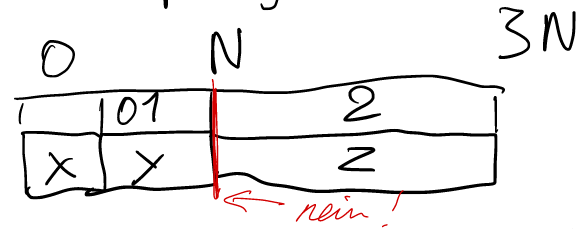
\includegraphics[width=\columnwidth]{img/pumpinglemma.png} \\
(Der OBERE strich zwischen 01 und 2 darf nicht auf Höhe des y strichs sein. Siehe brändli Spick) \\
5. Pumpen: Der y-Teil wird aufgepumpt Anzahl 01 verändert sich, Anzahl 2 bleibt gleich. $xy^k z \notin L$ $∀ k ≠ 2$ \\
6. Widerspruch -> L ist nicht regulär

